\documentclass[11pt]{article}
\usepackage[paper=letterpaper,margin=2cm]{geometry}
\usepackage{graphicx}
\usepackage{hyperref}
\usepackage{enumitem}
\usepackage{amsmath,amsfonts,amssymb}
\usepackage{array}
\usepackage[export]{adjustbox}

\graphicspath{ {./images/} }

\hypersetup{
    colorlinks,
    citecolor=black,
    filecolor=black,
    linkcolor=black,
    urlcolor=black
}

\def\arraystretch{1.5}
\newcolumntype{C}[1]{>{\centering\arraybackslash} m{#1} }

\setlength\parskip{1em plus 0.1em minus 0.2em}
\setlength\parindent{0pt}

\begin{document}

\begin{titlepage}
    \begin{center}
        \vspace*{1cm}

        \textbf{\LARGE Gestão}
        \vspace{0.5cm}

        \Large Resumo
        \vspace{1.5cm}

        \textbf{Rafael Rodrigues}
        \vfill
        LEIC \\
        Instituto Superior Técnico \\
        2023/2024
    \end{center}
\end{titlepage}

\tableofcontents

\newpage

\section{Introdução}

\subsection{Conceitos fundamentais sobre Gestão}

\textbf{Gestão -} processo que tem como função atingir as metas e objetivos de uma organização, de forma eficiente e eficaz.

\textbf{Eficiência -} atingir um objetivo com o mínimo de recursos.

\textbf{Eficácia -} atingir o objetivo.

\textbf{Organização -} entidade social direcionada por objetivos e (deliberadamente) estruturada.

\subsection{Funções da Gestão}

O processo de gestão divide-se em 4 funções:
\begin{itemize}[topsep=0pt]
    \item \textbf{Planeamento -} Definir objetivos e ações. Decidir que tarefas serão executadas e alocar recursos para as mesmas e calendarizá-las.
    \item \textbf{Organização -} Designa e agrupa tarefas, alocando-as às várias estruturas da organização.
    \item \textbf{Liderança -} Utilizar influência para gerir o estado emocional do corpo trabalhador para atingir os objetivos da organização.
    \item \textbf{Controlo -} Monitorizar atividades do corpo trabalhador, determinar se a organização se está a aproximar dos objetivos e fazer correções quando necessário.
\end{itemize}

\subsection{Competências de um Gestor}

\begin{itemize}
    \item \textbf{Conceptuais -} capacidade de ver (e agir na) a organização como um todo (componentes e relações entre elas) e estabelecer as relações com o exterior. Requer a capacidade de pensar estrategicamente. Fundamental na gestão de topo.
    \item \textbf{Humanas -} capacidade em trabalhar com outras pessoas quer individualmente quer em equipa. Fundamental na gestão de topo e intermédia.
    \item \textbf{Técnicas -} domínio de tarefas específicas (métodos, técnicas, outros conhecimentos). Têm menor peso na gestão de topo.
\end{itemize}

\subsection{Ética}

Código de princípios morais e valores que governam o comportamento de uma pessoa ou organização, pronunciando-se sobre o que está certo ou errado.

A ética pertence à cultura de uma organização, e tem implicações diretas sobre a responsabilidade social (interna e externa) da empresa.

\subsection{Responsabilidade Social}

Responsabilidade dos gestores de fazer escolhas e promover ações que contribuem para os interesses comuns da sociedade e organização. Nomeadamente:
\begin{itemize}[topsep=0pt]
    \item Cumprimento das Leis Laborais e proteção dos trabalhadores
    \item Cumprimento das Leis Ambientais
    \item Responsabilidade perante os detentores de interesses
    \item Concorrência leal com as outras empresas
    \item Respeito para com os consumidores
    \item Relacionamento com Fornecedores
    \item Atividades em benefício da sociedade ou comunidades
\end{itemize}

\subsection{Estrutura Organizacional}

Conjunto de tarefas formais atribuídas a entidades da empresa (indivíduos, equipas e departamentos) conjugados com as linhas de autoridade, ónus de decisão e hierarquias, incluindo ainda sistemas de coordenação e controlo.

\subsubsection{Tipos de Estrutura}

\begin{tabular}{ | C{90pt} | C{100pt} | C{150pt} | }
    \hline
    Tipo de Estrutura & Vantagens                              & Desvantagens                                             \\\hline
    Funcional         & especialização, economias de escala    & fraca comunicação entre departamentos                    \\\hline
    Divisional        & flexibilidade, adaptação               & duplicação de recursos, fraca coordenação entre divisões \\\hline
    Matricial         & interdisciplinaridade                  & conflitos na cadeia de comando                           \\\hline
    Em Equipa         & rapidez de resposta, entusiasmo        & tempo em reuniões, conflitos eventuais                   \\\hline
    Rede              & flexibilidade, poucos custos estrutura & coordenação e controlo mais difícil                      \\\hline
\end{tabular}

\newpage

\section{Informação Financeira}

\textbf{Contabilidade -} Processo formal de identificar, medir e comunicar informação sobre o património e resultados de uma empresa para os níveis de decisão internos ou agentes externos.

\subsection{Organização da Informação Financeira}

\begin{itemize}
    \item Contabilidade Geral (Financeira ou Externa)
          \begin{itemize}
              \item Gera informação para os elementos externos à empresa         (reguladores, fornecedores, acionistas, bancos, etc.).
              \item Segue as normas internacionais de contabilidade em vigor.
              \item O Sistema de Normalização Contabilística assimila a
                    transposição das diretivas contabilísticas da União Europeia.
          \end{itemize}
    \item Contabilidade Analítica (de Gestão ou Interna)
          \begin{itemize}
              \item Gera informação específica e desagregada para apoiar a gestão.
              \item Apura resultados por produtos, regiões, mercados, atividades, etc.
              \item É a base para a orçamentação e análise de custos.
          \end{itemize}
\end{itemize}

\subsection{Principais Mapas Contabilísticos}

\subsubsection{Balanço}

O balanço permite registar as contas de um agente económico. É composto por 3 grandes rubricas, que depois podem ser distinguidas em sub-partes:

\begin{itemize}[topsep=0pt]
    \item \textbf{Ativo -} Bens e direitos que a empresa possui ou tem direito a receber.
          \begin{itemize}[topsep=0pt]
              \item \textbf{Ativo não Corrente -} Ativo que por natureza, não é volátil.
                    \begin{itemize}
                        \item \textbf{Ativos Fixos Tangíveis} (Edifícios, equipamentos, ...)
                        \item \textbf{Ativos Intangíveis} (Marcas, patentes, ...)
                    \end{itemize}
              \item \textbf{Ativo Corrente -} Ativos voláteis.
                    \begin{itemize}
                        \item \textbf{Inventários} (Produtos fabricados, em vias de fabricação ou matéria prima)
                        \item \textbf{Valores Monetários} (Dinheiro, depósitos e títulos financeiros)
                        \item \textbf{Dívidas de clientes}
                    \end{itemize}
          \end{itemize}
    \item \textbf{Passivo -} Soma das dívidas (responsabilidades) de um agente económico.
          \begin{itemize}[topsep=0pt]
              \item \textbf{Passivo não Corrente -} Financiamentos e outras dívidas (a pagar em mais de 1 ano)
              \item \textbf{Passivo Corrente -} Dívida a fornecedores, estado, financiamentos ou outras (a pagar em menos de 1 ano)
          \end{itemize}
    \item \textbf{Capital Próprio -} Capital realizado e lucros do período ou de períodos anteriores retidos na empresa.
\end{itemize}

\newpage

\subsubsection*{Equação Fundamental da Contabilidade}

\begin{center}
    \textbf{Ativo = Passivo + Capital Próprio}
\end{center}

Se Ativo $>$ Passivo $\implies $ Capital Próprio $>$ 0 \\
Se Ativo $<$ Passivo $\implies $ Capital Próprio $<$ 0 (falência técnica)

\subsubsection{Demonstração dos Fluxos de Caixa}

\textbf{Ótica da Caixa -} Permite ver o dinheiro que uma empresa tem num determinado momento, a Liquidez.
\begin{center}
    Saldo inicial + Dinheiro recebido + Pagamentos = Saldo Final
\end{center}

\subsubsection{Demonstração de Resultados}

\textbf{Ótica de Exercício -} Permite ver se a empresa é rentável.

\begin{center}
    Rendimentos - Gastos = Resultado Líquido do Período
\end{center}

\begin{center}
    Demonstração de Resultados \\
    \begin{tabular}[t]{ | p{250pt} | }
        \hline Valor das vendas                                                   \\
        \hline Custo das vendas                                                   \\
        \hline \multicolumn{1}{ |r| }{\textbf{Resultado Bruto (RB)}}              \\
        \hline Outros Rendimentos                                                 \\
        \hline Outros Gastos                                                      \\
        \hline \multicolumn{1}{ |r| }{\textbf{Resultado Operacional (RO)}}        \\
        \hline Juros                                                              \\
        \hline \multicolumn{1}{ |r| }{\textbf{Resultado Antes de Impostos (RAI)}} \\
        \hline Impostos                                                           \\
        \hline \multicolumn{1}{ |r| }{\textbf{Resultado Líquido (RL)}}            \\
        \hline
    \end{tabular}
\end{center}

\newpage

\subsection{Análise de Rácios Financeiros}

\textbf{Rácios -} Indicadores de gestão que exprimem uma relação entre elementos dos documentos contabilísticos (Balanço, Demonstração de Resultados) e a partir dos quais é possível tirar ilações sobre a situação da empresa (Solidez Financeira e níveis de desempenho económico e financeiro).


Dizemos que uma empresa tem \textbf{Solidez Financeira}:
\begin{itemize}
    \item Quanto maior o capital próprio e menor o passivo (melhor ainda se o passivo for não corrente).
    \item Quanto maior for o somatório do capital próprio com o passivo não corrente, relativamente ao ativo corrente.
    \item Quanto maior a rentabilidade do capital total em relação ao juro a pagar pelo capital alheio.
\end{itemize}

\subsubsection{Rácios de Rentabilidade}

Indicam a rentabilidade do capital próprio, ativo ou vendas.

\begin{equation*}
    \textrm{Rentabilidade do Capital Próprio (RCP)} =
    \frac{\textrm{Resultado Líquido}}{\textrm{Capital Próprio}}
\end{equation*}

\begin{equation*}
    \textrm{Rentabilidade das Vendas} =
    \frac{\textrm{Resultado Operacional}}{\textrm{Vendas}}
\end{equation*}

\subsubsection{Rácios de Atividade ou Funcionamento}

Indicam o grau de utilização dos recursos da empresa.

\begin{equation*}
    \textrm{Prazo Médio de Recebimentos (em dias)} =
    \frac{\textrm{Clientes}}{\textrm{Vendas}} \times 365
\end{equation*}

\begin{equation*}
    \textrm{Prazo Médio de Pagamentos (em dias)} =
    \frac{\textrm{Fornecedores}}{\textrm{Compras}} \times 365
\end{equation*}

\begin{equation*}
    \textrm{Rotação de Inventários} =
    \frac{\textrm{Custo das Vendas}}{\textrm{Inventários médios}}
\end{equation*}

\subsubsection{Rácios de Solvabilidade}

Indicam a capacidade da empresa de satisfazer os compromissos financeiros de médio e longo prazo.

\begin{equation*}
    \textrm{Solvabilidade Total (Autonomia Financeira)} =
    \frac{\textrm{Capital Próprio}}{\textrm{Ativo}}
\end{equation*}

Uma boa solvabilidade total corresponde a valores acima de 1/3.

\begin{equation*}
    \textrm{Solvabilidade Reduzida} =
    \frac{\textrm{Capital Próprio}}{\textrm{Passivo}}
\end{equation*}

Uma boa solvabilidade reduzida corresponde a valores acima de 1/2.

\subsubsection{Rácios de Liquidez}

Indicam a capacidade de a empresa satisfazer os compromissos financeiros de curto prazo através do fundo de maneio.

\textbf{Fundo de maneio -} diferenca entre Ativo Corrente e Passivo Corrente.

\begin{equation*}
    \textrm{Liquidez Geral} =
    \frac{\textrm{Ativo Corrente}}{\textrm{Passivo Corrente}} =
    \frac{\textrm{Caixa + Clientes + Inventário}}{\textrm{Passivo Corrente}}
\end{equation*}

\begin{equation*}
    \textrm{Liquidez Reduzida} =
    \frac{\textrm{Ativo Corrente - Inventário}}{\textrm{Passivo Corrente}} =
    \frac{\textrm{Caixa + Clientes}}{\textrm{Passivo Corrente}}
\end{equation*}

\subsection{Análise Custo-Volume-Resultado}

\textbf{Custos Fixos -} Gastos em que a empresa incorre independentemente da quantidade produzida (ex: Gastos de instalação).

\textbf{Custos Variáveis -} Variam proporcionalmente com a quantidade produzida (ex: custos de matéria-prima).

\textbf{Ponto Crítico -} Nível de atividade que corresponde a Lucro zero, ou seja, a quantidade produzida a partir do qual a empresa passa a ter lucro (ou seja, passa a ser rentável).

\begin{minipage}[b]{0.5\textwidth}
    \begin{align*}
        Lucro = 0 & \implies p * Q - CV - CF = 0       \\
                  & \implies p * Q - cv_u * Q - CF = 0 \\
                  & \implies (p - cv_u) * Q - CF = 0   \\
                  & \implies mc_u * Q = CF
    \end{align*}
\end{minipage}
\begin{minipage}[b]{0.49\textwidth}
    $Q$ - Quantidade produzida e vendida         \\
    $p$ - Preço de venda unitário                \\
    $CV$ - Total dos Custos Variáveis            \\
    $CF$ - Total dos Custos Fixos                \\
    $cv_u$ - Custo variável unitário (constante)
\end{minipage}

\vspace{10pt}

\begin{minipage}{0.5\textwidth}
    \begin{equation*}
        mc_u = p - cv_u
    \end{equation*}
\end{minipage}
\begin{minipage}{0.49\textwidth}
    $mc_u$ - Margem de contribuição unitária
\end{minipage}

\begin{minipage}{0.5\textwidth}
    \begin{equation*}
        Q_c = \frac{CF}{mc_u}
    \end{equation*}
\end{minipage}
\begin{minipage}{0.49\textwidth}
    $Q_c$ - Quantidade crítica a partir da qual há lucro
\end{minipage}

\begin{minipage}{0.5\textwidth}
    \begin{equation*}
        R_c = p \times Q_c
    \end{equation*}
\end{minipage}
\begin{minipage}{0.49\textwidth}
    $R_c$ - Receita crítica a partir da qual há lucro
\end{minipage}

\newpage

\section{Análise de Projetos de Investimento}

\textbf{Investimento -} Aplicação de recursos, com vista em obter retorno futuro.

\subsection{Como calcular valores atuais e futuros}

\subsubsection{Juro}

Remuneração cobrada pelo empréstimo de dinheiro (ou outro item).
\begin{itemize}[topsep=0pt]
    \item \textbf{Juro Simples: }$C_i\times (1+r)$
    \item \textbf{Juro Composto} (no ano inicial $i=0$)
          \begin{itemize}
              \item \textbf{Capitalização: }$C_n=C_i\times(1+r)^{n-i}$
                    \ \ (capital na $n$-ésima iteração)
              \item \textbf{Atualização: }$\displaystyle C_i=\frac{C_n}{(1+r)^{n-i}}$
                    \ \ (capital no ano $i$, baseado no valor atual)
          \end{itemize}
\end{itemize}

\subsubsection{Taxas de Juro}

\textbf{Taxa de Juro Nominal ($r_n$) -} usa-se na avaliação de projetos a preços correntes, não está ajustada à inflação.

\textbf{Taxa de Juro Real ($r_r$) -} usa-se na avaliação de projetos a preços constantes, ajustada à inflação ($i$).
\begin{equation*}
    r_r = \frac{1+r_n}{1+i} - 1 \approx r_n - i
\end{equation*}

\textbf{Taxa Anual Nominal (TAN) -} seja $r_a$ uma taxa de juro anual. A taxa mensal \textbf{proporcional} é:
\begin{equation*}
    r_{mp} = \frac{r_a}{12}
\end{equation*}

\textbf{Taxa Anual Efetiva (TAE) -} seja $r_a$ uma taxa de juro anual. A taxa mensal \textbf{equivalente} é:
\begin{equation*}
    \displaystyle r_{me} = (1+r_a)^{\frac{1}{12}} - 1
\end{equation*}
Dada um taxa de juro mensal, podemos também calcular a TAE correspondente:
\begin{equation*}
    \displaystyle r_{ae} = (1+r_m)^{12} - 1
\end{equation*}

\textbf{Equivalência de Taxas de Juro -} Duas taxas de juro dizem-se equivalentes se a sua aplicação corresponde ao mesmo valor, ao fim do mesmo período de tempo.
\begin{equation*}
    (1+r_k)^k = 1 + r_a
\end{equation*}

\subsubsection{Anuidade}

Pagamento que é feito repetidamente, durante $n$ períodos. Seja $r$ a taxa de atualização, ou seja, o valor pelo qual se atualiza o pagamento, a cada iteração. Seja $A$ o valor da anuidade.
\begin{itemize}[topsep=0pt]
    \item Valor do $i$-gésimo pagamento: $\displaystyle p_i=A\frac{1}{(1+r)^i}$
    \item Valor atual (soma das anuidades): $\displaystyle VA=A\frac{(1+r)^n-1}{(1+r)^n\times r}=Af(r,n)$\\[6pt]
          A $f(r,n)$ chamamos \textbf{fator de anuidade}. Quando $\displaystyle n = \infty \Rightarrow f(r,\infty)=\frac{1}{r}$
\end{itemize}

\subsection{Análise da Rentabilidade de Projetos de Investimento}

\textbf{Cash Flow -} Fluxo financeiro, pode ser positivo ou negativo.

\textbf{Investimento -} Podemos redefinir um investimento como uma sequência de cash flows distribuídos no tempo, onde os primeiros são tipicamente negativos (despesa de investimento).

\subsubsection{Valor Residual do Investimento (VR)}

Valor gerado pela venda de um ativo fixo no final do projeto de investimento.
\begin{equation*}
    VR = VM - (VM - VC) \times \text{Taxa de Imposto}
\end{equation*}
VM - Valor de Mercado (esperado de venda do ativo no ano $n$) \\
VC = Valor de Compra $-$ Deprec./Amortiz. acumuladas (valor contabilístico)

\subsubsection{Cash-Flows de Exploração}

Os cash-flows durante a fase de exploração (passada a fase inicial de investimento) serão habitualmente positivos se o projeto for lucrativo.
\begin{equation*}
    \text{CF Exploração} =
    RO \times (1 - \text{Taxa de Imposto}) + \text{Deprec./Amortiz.}
\end{equation*}

\subsubsection{Atualizações}

Depois de obter o Cash-Flow de Exploração conseguimos calcular o Cash-Flow total:
\begin{center}
    Cash-Flow Total = Cash-Flow do Investimento + Cash-Flow de Exploração
\end{center}

Devemos depois calcular o seu valor atualizado à taxa $r$ para cada ano ($n$) :
\begin{equation*}
    \text{Cash-Flow Atualizado} = \frac{\text{Cash-Flow Total}}{(1+r)^n}
\end{equation*}

\subsubsection{Custo Médio Ponderado do Capital (CMPC)}

\begin{equation*}
    CMPC =
    \frac{D}{C_{total}}\times r_D\times(1-t)+\frac{CP}{C_{total}}\times r_{CP}
\end{equation*}
$t$ - taxa de imposto \\
$r_D$ - taxa de juro da dívida (custo médio da dívida) \\
$r_{CP}$ - taxa de remuneração dos acionistas + prémio de risco

\subsubsection{Valor Atual Líquido (VAL)}

Soma de todos os $CF$ (cash-flow) do projeto devidamente atualizados à taxa $r$.
\begin{equation*}
    \text{VAL}(r) = \sum \frac{CF_K}{(1+r)^K}
\end{equation*}
Um projeto é rentável se VAL $>$ 0.
Para dois projetos, se VAL$_A >$ VAL$_B$ então $P_A$ é melhor que $P_B$.

\subsubsection{Taxa Interna de Rentabilidade (TIR)}

Valor da taxa de atualização ($r$) para a qual o VAL = 0. O projeto é rentável se TIR $>$ R.

\subsubsection{Período de Recuperação do Investimento (PRI)}

Tempo necessário para que os cash-flows (atualizados a $r$) gerados pelo projeto igualem o capital investido inicialmente.
\begin{equation*}
    \sum_{K=0}^{PRI} \frac{CF_K}{(i+r)^K}=0
\end{equation*}
\begin{equation*}
    PRI = K_{\text{último CF acumulado negativo}} - \frac{\text{último CF}_{\text{acumulado negativo}}}{\text{CF}_{\text{atualizado}}\text{ de K}_{\text{primeiro CF acumulado positivo}}}
\end{equation*}

\subsubsection{Índice de Rendibilidade (IR)}

Métrica para medir a rentabilidade de um investimento. Considera-se aceitável quando IR $>$ 1.
\begin{equation*}
    \text{IR} = \frac{\text{VAL + Investimento Inicial}}{\text{Investimento Inicial}}
    = \frac{\text{VA}}{\text{Investimento Inicial}}
\end{equation*}

\newpage

\section{Gestão Estratégica}

\subsection{Processo de Formulação e Execução da Estratégia}

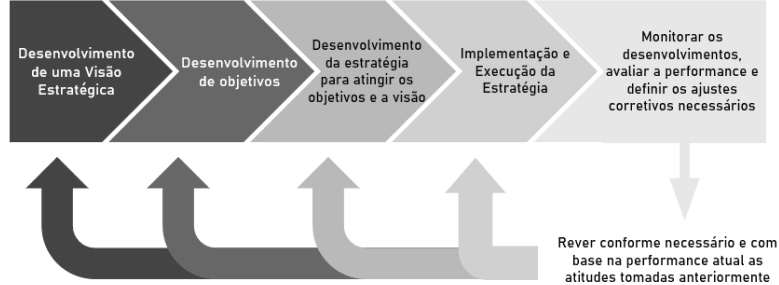
\includegraphics[width=\textwidth]{gestao_estrategica.png}

\subsubsection{Visão}

A visão centra-se no \textbf{futuro} e estabelece uma direção de longo prazo. É elaborada pela \textbf{gestão de topo} de uma organização, comunicada posteriormente aos investidores e às camadas inferiores da hierarquia.

\subsubsection{Objetivos}

Os objetivos convertem a visão (que é abstrata) em \textbf{alvos de desempenho} específicos e permitem monitorar o desempenho da organização.

São transversais a toda a estrutura organizacional, sendo estabelecidos de uma forma descendente, mas de forma colaborativa, de modo a garantir que os objetivos estabelecidos para níveis inferiores apoiam os objetivos dos níveis superiores.

Os objetivos devem:
\begin{itemize}[topsep=-4pt,itemsep=0pt]
    \item ser quantificáveis
    \item ser mensuráveis
    \item ter um prazo para serem atingidos
\end{itemize}

\subsection{Análise Estratégica}

O objetivo da análise estratégica é obter informação que permita ajudar a organização a desenhar/formular uma estratégia adequada.

\subsection{Formulação da Estratégia}

A Formulação da Estratégia pode ser dividida em 4 níveis:
\begin{itemize}[topsep=0pt]
    \item \textbf{Estratégia Corporativa} - em que sectores a empresa deve estar.
    \item \textbf{Estratégia Negocial} - como queremos construir uma vantagem competitiva.
    \item \textbf{Estratégia Funcional} - como deve ser, detalhadamente, implementada a  estratégia de negócio.
    \item \textbf{Estratégia Operacional}
\end{itemize}

\subsubsection{Estratégias ao Nível Corporativo}

\subsubsection*{Concentração vs. Diversificação}

Uma organização pode concentrar-se num negócio ou diversificar-se em mais que um. Esta diversificação pode estar relacionada com os negócios existentes ou não.
É preciso saber se é possível capturar sinergias entre as diferentes áreas de negócio.
Para além disso é preciso analisar as prioridades de investimento e de alocação da organização.

\begin{minipage}{0.5\textwidth}
    \textbf{Matriz BCG}:
    \begin{itemize}
        \item \textbf{Cash-Cow}: Setor que já não está em crescimento, mas o produto fabricado é o mais vendido (líder de mercado).
        \item \textbf{Star}: O setor está em crescimento e o seu produto é o mais vendido.
        \item \textbf{Question-Marks}: O setor está num mercado em crescimento, mas o seu produto não é o mais vendido.
        \item \textbf{Dog}: O setor não está em crescimento e também não tem uma posição dominante no mercado.
    \end{itemize}
\end{minipage}
\begin{minipage}{0.49\textwidth}
    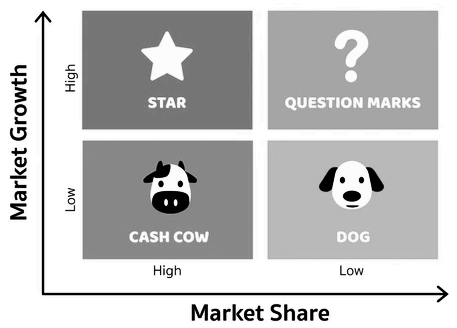
\includegraphics[scale=0.65,right]{matriz_BCG.png}
\end{minipage}


\subsubsection*{Integração vertical}

Visa a criação de valor através:
\begin{itemize}[topsep=0pt]
    \item da produção própria dos “inputs” necessários (backward vertical integration)
    \item da distribuição própria dos produtos produzidos pela empresa (forward
          vertical integration)
    \item \textbf{Vantagens}: reduz custos e diminui a dependência.
    \item \textbf{Desvantagens}: aumenta a necessidade de recursos e coordenação, e diminui a flexibilidade (se o produto tiver de mudar as matérias primas, perde-se uma estrutura que já está criada)
\end{itemize}

\subsubsection{Estratégias ao Nível do Negócio}

\begin{itemize}
    \item \textbf{Liderança de Baixo-Custo}: através da prática de custos muito baixos (utilizando técnicas difíceis de copiar) conseguir uma grande cota de mercado.
    \item \textbf{Diferenciação}: através de produtos únicos, conseguir a preferência do mercado.
    \item \textbf{Diferenciação em Nicho}: servir um segmento específico, sendo dominante nesse nicho através da diferenciação
    \item \textbf{Baixo-Custo em Nicho}: servir um segmento específico, sendo dominante nesse nicho através da prática de preços baixos.
    \item \textbf{Relação Custo-Qualidade}: tentar criar o melhor produto a um preço baixo, conseguindo manter a qualidade mas cativando clientes que valorizam preços em conta.
\end{itemize}

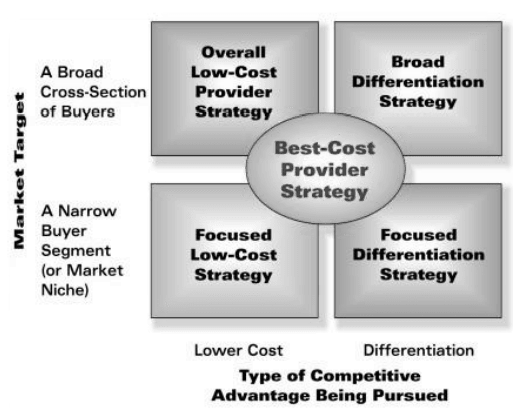
\includegraphics[scale=0.8,center]{estrategia-nivel-negocio.png}

\newpage

\section{Marketing}

Atividade que reúne os processos para criar, comunicar, entregar e trocar ofertas que fornecem valor a clientes, parceiros e à sociedade em geral.

\subsection{Conceitos Fundamentais}

Filosofias das Organizações na abordagem ao Mercado:
\begin{itemize}[topsep=0pt]
    \item \textbf{Produção} - Os consumidores privilegiam produtos largamente disponíveis e baratos.\\[4pt]
          $\Rightarrow$ Eficiência, custos baixos, produção em massa.
    \item \textbf{Produto} - Os consumidores preferem produtos com a melhor qualidade, desempenho e inovação.\\[4pt]
          $\Rightarrow$ Excelência, qualidade.
    \item \textbf{Venda} - Os consumidores não mostram iniciativa em comprar.\\[4pt]
          $\Rightarrow$ Pro-atividade, força de vendas, promoção.
    \item \textbf{Marketing} - O foco não deve ser no produto mas na ação de satisfazer uma necessidade/processo.\\[4pt]
          $\Rightarrow$ Encontrar o produto adaptado a essas necessidades.
    \item \textbf{Marketing Social} (societal marketing) - Marketing em que existe a preocupação com o bem-estar dos consumidores e da sociedade.
\end{itemize}

\subsection{Segmentação, Targeting e Posicionamento (STP)}

\textbf{Marketing Indiferenciado} - Nesta variante (mais antiga) procura-se vender o mesmo produto a todos os consumidores.

\textbf{Marketing Diferenciado} - Procura-se personalizar um produto para diferentes segmentos-alvos do mercado.

\subsubsection{Segmentação}

Consiste em identificar as variáveis que tornem possível a separação do mercado em segmentos.

Uma boa segmentação separa os consumidores em segmentos onde há diferenças substanciais que os distingam.

A segmentação pode ser feita por:
\begin{itemize}[topsep=0pt]
    \item \textbf{Características} - que podem ser geográficas, demográficas ou psicográficas.
    \item \textbf{Comportamentos} - como tirar vantagem de ocasiões, de benefícios pretendidos ou de frequência de utilização do produto.
\end{itemize}

\subsubsection{Targeting}

Avaliar a atratividade de cada segmento, de modo a escolher os segmentos-alvo.
\begin{itemize}[topsep=0pt]
    \item \textbf{Marketing concentrado}: escolher um único segmento-alvo
    \item \textbf{Especialização seletiva}: Cobertura de vários segmentos-alvo
    \item \textbf{Cobertura total}: dos segmentos do mercado
\end{itemize}

\subsubsection{Posicionamento}

Para cada segmento alvo, saber identificar como o produto é importante para
o consumidor e como se diferencia da competição.

\subsection{Marketing Mix}

\subsubsection{Produto}

\textbf{Produto} - Tudo que pode ser oferecido a um mercado para aquisição, atenção, uso ou consumo, e que possa satisfazer uma necessidade ou desejo.

Ciclo de vida de um produto:
\begin{itemize}[topsep=0pt]
    \item Desenvolvimento: não está disponível ao público, incorre-se em prejuízo
    \item Introdução: é colocado no mercado
    \item Crescimento: começa a dar lucros
    \item Maturidade: estabiliza a receita oferecida
    \item Declínio: diminui a receita
\end{itemize}


\textbf{Serviço} - Ato que é oferecido numa transação. Contém as seguintes características:
\begin{itemize}[topsep=0pt]
    \item Intangibilidade: não é um bem físico.
    \item Inseparabilidade: necessidade de estar presente na altura e local da prestação do serviço
    \item Variabilidade: atendimento diferente por duas pessoas ou pela mesma em
          diferentes alturas
    \item Perecibilidade: não é possível armazenar o que não foi comprado
\end{itemize}

\subsubsection{Preço}

O preço é o motor do rendimento que um produto traz. A definição do preço de um produto, entre os limites mínimo (custo de produção) e máximo (valor percetual para o cliente) depende dos preços da concorrência, do segmento de mercado e do posicionamento pretendido.

Estratégias para estabelecer o \textbf{preço de um novo produto}:
\begin{itemize}[topsep=0pt]
    \item \textbf{Skimming} (desnatação) - Colocar o produto a um preço alto e ir diminuindo mediante a resposta de mercado.
    \item \textbf{Penetração} - Colocar o produto a um preço baixo e ir aumentando mediante a resposta de mercado.
\end{itemize}

Para estabelecer o preço de um produto já existente devemos considerar a sua \textbf{perecibilidade}, \textbf{grau de diferenciação} e \textbf{estágio do ciclo de vida} em que se encontra.

\subsubsection{Distribuição}

Processo de levar um produto/serviço às pessoas certas no tempo certo, considerando o lucro e a eficácia.

Os circuitos de distribuição podem ter vários níveis, quanto maior o número de intermediários entre o produtor e consumidor, maior o nível.

Tipos de distribuição (em função do nível):
\begin{itemize}[topsep=0pt]
    \item \textbf{Distribuição exclusiva} \\
          Apenas uma ou muito poucas lojas de uma pequena cadeia, restringindo o número por área geográfica - por exemplo venda de produtos Gucci através das lojas daquela marca.
    \item \textbf{Distribuição seletiva} \\
          Apenas alguns intermediários, para manter controlo, por exemplo, sobre o tipo de serviço - por exemplo certos modelos de televisores podem ser vendidos apenas através de certas cadeias de lojas.
    \item \textbf{Distribuição intensiva} \\
          Em muitos pontos de distribuição - frequentemente associada a bens de conveniência, tais como refrigerantes, massas, arroz, jornais.
\end{itemize}

\subsubsection{Comunicação/Promoção}

Conjunto de atividades desenvolvidas pela empresa para comunicar com os seus clientes - atuais e potenciais.

Principais componentes da comunicação/promoção:
\begin{itemize}[topsep=0pt]
    \item \textbf{Publicidade -} Forma paga de apresentação e de comunicação não pessoal de organizações, ideias, bens ou serviços, efetuada por um patrocinador identificado, para uma audiência alvo, através de um meio de comunicação de massas.
    \item \textbf{Promoção de Vendas -} Incentivos de curto prazo e temporários destinados a encorajar experimentação ou compra (ou recompra) de um bem ou serviço.
    \item \textbf{Força de Vendas -} Interação pessoal com compradores (correntes e potenciais).
    \item \textbf{Marketing Direto -} Comunicação ou solicitação direta da atuação de clientes atuais e potenciais específicos utilizando o correio, telefone, e-mail ou outros meios não pessoais.
    \item \textbf{On-line, social media e mobile marketing -} Atividades on-line e programas desenhados para envolver clientes atuais ou potenciais: websites, comunidades on-line, blogs e redes sociais como Facebook e Twitter, mensagens de texto e apps para smartphones e tablets.
    \item \textbf{Relações Públicas -} Programas destinados a promover e/ou proteger a imagem da organização ou dos seus produtos.
    \item \textbf{Eventos e Experiências -} Eventos e experiências são atividades e programas patrocinados e concebidos para criar interações diárias ou especiais com marcas.
\end{itemize}

\subsection*{Estratégias Push e Pull}

\begin{itemize}[topsep=0pt,itemsep=0pt]
    \item Estratégia Push \\
          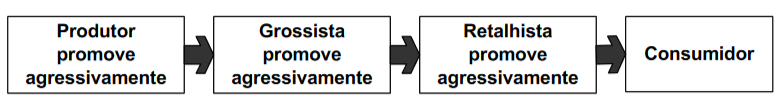
\includegraphics[width=13cm]{estrategia_push.png}
    \item Estratégia Pull \\[5pt]
          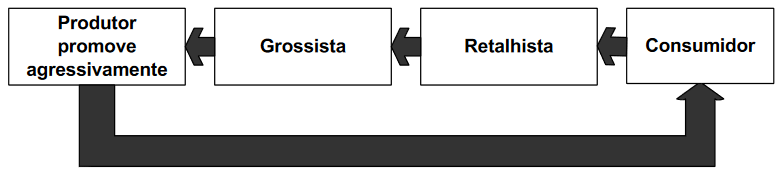
\includegraphics[width=13cm]{estrategia_pull.png}
\end{itemize}

\subsection*{Resumo}

Marketing típico em cada fase do ciclo de vida, embora esteja longe de universalmente aplicável.

\begin{tabular}{ C{2.1cm} | C{3.3cm} | C{3.3cm} | C{3.3cm} | C{3.3cm} }
                           & Introdução                                                                                                                 & Crescimento                                                                          & Maturidade                                                                                                            & Declínio                                                                \\\hline
    Objetivos de Marketing & Criar consciência e experimentação                                                                                         & Maximizar de quota de mercado                                                        & Maximizar lucro defendendo quota de mercado                                                                           & Reduzir despesas e retirar o máximo de valor                            \\\hline
    Produto                & Produto básico                                                                                                             & Oferecer extensões, serviços, garantias                                              & Diversificar marcas e modelos                                                                                         & Abandonar itens mais fracos                                             \\\hline
    Preço                  & Baseado no custo *                                                                                                         & Penetração *                                                                         & Face à concorrência                                                                                                   & Baixar preço **                                                         \\\hline
    Distribuição           & Seletiva                                                                                                                   & Intensiva                                                                            & Mais intensiva                                                                                                        & Evoluir para seletiva                                                   \\\hline
    Promoção               & Publicidade/vendas pessoais para criar consciência nos inovadores e distribuidores; Promoção de vendas para experimentação & Publicidade/vendas pessoais para consciência e interesse Promoção de vendas reduzida & Publicidade/vendas pessoais para dar ênfase a diferenças de marca e benefícios Promoção de vendas para troca de marca & Reduzir a níveis mínimos (indispensáveis para retenção de núcleo  duro) \\
\end{tabular}

\end{document}